\section{Klein-Gordon equation}

As discussed previously, the Schrödinger equation arises from the quantization of a \textit{non-relativistic} particle.
In complete analogy, the \textbf{Klein–Gordon equation} can be obtained by applying the same quantization procedure to a \textit{relativistic} particle (this is often referred to as \textit{first quantization} of the relativistic theory).

However, unlike the Schrödinger equation, the Klein–Gordon equation does not allow for a consistent \textbf{probabilistic interpretation} in terms of a positive-definite probability density.
This limitation signals that the equation, while formally correct as a relativistic wave equation, cannot be the final description of a single-particle quantum system.

A consistent framework is recovered by interpreting the Klein–Gordon \textit{wave function} as a \textbf{classical field} and quantizing this field itself.
In this approach—known as \textbf{second quantization} or \textbf{field quantization}—the field is promoted to an operator acting on a Fock space, describing states with an arbitrary number of identical particles and antiparticles.
Historically, this formalism first appeared in the quantization of the electromagnetic field, and it naturally extends to the Klein–Gordon field.

In the language of quantum field theory, the Klein–Gordon field thus represents a system of \textbf{spin-0 particles} and their corresponding antiparticles.
Nevertheless, even if we restrict ourselves to the first-quantized formulation, the Klein–Gordon equation remains of fundamental importance, as it encapsulates the essential features of the quantum mechanics of relativistic scalar particles and provides the starting point for the construction of quantum field theory.

\subsection{Derivation of the Klein-Gordon equation}

How can we obtain a relativistic version of the wave equation?
A natural starting point is to repeat the same procedure used for the Schrödinger equation, but now employing the \textbf{relativistic energy–momentum relation}.
For a free relativistic particle of mass \( m \), the four-momentum \( p^\mu = (p^0, p^1, p^2, p^3) = (E, \mathbf{p}) \) satisfies the \textbf{mass-shell condition}
\[
    p^\mu p_\mu = -m^2 c^2 \quad \Rightarrow \quad E^2 = \mathbf{p}^2 c^2 + m^2 c^4.
\]

One could then try to promote this classical relation to a wave equation by using the correspondence
\[
    E \rightarrow i\hbar \frac{\partial}{\partial t},
    \qquad
    \mathbf{p} \rightarrow -i\hbar \nabla.
\]
If we apply this substitution directly to the relativistic energy expression \( E = \sqrt{\mathbf{p}^2 c^2 + m^2 c^4} \), we obtain
\[
    i\hbar \frac{\partial}{\partial t} \psi(\mathbf{x},t)
    = \sqrt{-\hbar^2 c^2 \nabla^2 + m^2 c^4} \, \psi(\mathbf{x},t).
\]
However, this equation involves the \textit{square root of a differential operator}, whose precise meaning is not well defined.
Such an operator would introduce \textbf{non-local effects}, implying that distant points in space could directly influence each other—an undesirable and physically obscure feature.
For this reason, this form was soon abandoned.

A more elegant and mathematically tractable approach was proposed independently by \textbf{Oskar Klein} and \textbf{Walter Gordon}.
Instead of working with the square-root form, they started from the \textit{quadratic} energy–momentum relation
\[
    E^2 = \mathbf{p}^2 c^2 + m^2 c^4,
\]
and replaced \( E \) and \( \mathbf{p} \) by their corresponding operators.
This leads to the \textbf{Klein–Gordon equation}:
\begin{equation}
    \left( -\frac{1}{c^2} \frac{\partial^2}{\partial t^2} + \nabla^2 - \frac{m^2 c^2}{\hbar^2} \right) \psi(\mathbf{x},t) = 0.
\end{equation}
In a more compact and manifestly relativistic form, it can be written as
\begin{equation}
    (\Box - m^2) \, \phi(x) = 0,
\end{equation}
where the \textbf{d'Alembertian operator} is defined as
\[
    \Box = \partial^\mu \partial_\mu = -\partial_0^2 + \nabla^2.
\]

From now on, we adopt \textbf{natural units} with \( \hbar = c = 1 \), so that the equation takes the simple form
\[
    (\Box - m^2)\phi = 0,
\]
and the mass \( m \) becomes dimensionless, unless otherwise specified.

\subsection{Plane wave solutions}

The Klein–Gordon equation was constructed precisely to ensure that it admits plane-wave solutions satisfying the correct relativistic dispersion relation between energy and momentum:
\[
    (\Box - m^2)\,\phi(x) = 0.
\]

To find such solutions, let us assume a \textbf{plane wave ansatz} of the form
\begin{equation}
    \phi_p(x) = e^{i p_\mu x^\mu},
\end{equation}
where \( p_\mu \) is the four-momentum of the particle.
Substituting this expression into the Klein–Gordon equation gives
\[
    (\partial^\mu \partial_\mu - m^2)\, e^{i p_\nu x^\nu}
    = ((ip^\mu)(ip_\mu) - m^2)\, e^{i p_\nu x^\nu}
    = -(p^\mu p_\mu + m^2)\, e^{i p_\nu x^\nu} = 0.
\]
This condition is satisfied if the four-momentum \( p^\mu \) lies on the \textbf{mass shell}, that is,
\[
    p^\mu p_\mu = -m^2
    \quad \Rightarrow \quad
    (p^0)^2 = \mathbf{p}^2 + m^2
    \quad \Rightarrow \quad
    p^0 = \pm E_p, \qquad
    E_p = \sqrt{\mathbf{p}^2 + m^2}.
\]

Hence, the Klein–Gordon equation admits both \textbf{positive-} and \textbf{negative-energy solutions}.
The positive-energy modes correspond to
\[
    \phi(x) = e^{-i E_p t + i \mathbf{p} \cdot \mathbf{x}},
\]
while the negative-energy modes are given by
\[
    \phi(x) = e^{i E_p t - i \mathbf{p} \cdot \mathbf{x}}.
\]

At first sight, the existence of solutions with \( p^0 = -E_p \) seems problematic: if negative-energy states exist, the system could in principle decay indefinitely into lower and lower energy levels, making the theory \textbf{unstable}.
In the framework of relativistic quantum field theory, however, these modes acquire a consistent interpretation: they correspond to \textbf{antiparticles} carrying positive energy but opposite charge or quantum numbers.

The most general solution of the Klein–Gordon equation can therefore be expressed as a linear superposition of all plane waves with both signs of energy:
\begin{equation}
    \phi(x) = \int \frac{\mathrm{d}^3 \mathbf{p}}{(2\pi)^3 2E_p}
    \left[
        a(\mathbf{p})\, e^{-i E_p t + i \mathbf{p} \cdot \mathbf{x}}
        + b^*(\mathbf{p})\, e^{i E_p t - i \mathbf{p} \cdot \mathbf{x}}
        \right],
\end{equation}
and its complex conjugate as
\[
    \phi^*(x) = \int \frac{\mathrm{d}^3 \mathbf{p}}{(2\pi)^3 2E_p}
    \left[
        a^*(\mathbf{p})\, e^{i E_p t - i \mathbf{p} \cdot \mathbf{x}}
        + b(\mathbf{p})\, e^{-i E_p t + i \mathbf{p} \cdot \mathbf{x}}
        \right].
\]
Here, \( a(\mathbf{p}) \) and \( b(\mathbf{p}) \) are \textbf{Fourier coefficients} that determine the relative weight of each momentum mode.
The normalization factor \( 2E_p \) is conventional and chosen so that the coefficients transform as Lorentz scalars.
Finally, for a \textbf{real scalar field}, where \( \phi^* = \phi \), the coefficients of positive- and negative-energy modes coincide:
\[
    a(\mathbf{p}) = b(\mathbf{p}).
\]

\subsection{Continuity equation}

From the Klein–Gordon equation one can derive a continuity equation, although the associated conserved quantity cannot be interpreted as a probability density. Let us examine this in detail.

A straightforward way to obtain the continuity equation is to multiply the Klein–Gordon equation by the complex conjugate field $\phi^*$ and subtract from it the complex conjugate equation multiplied by $\phi$. One finds:
\[
    \begin{aligned}
        \phi^* (\Box - m^2) \phi - \phi (\Box - m^2) \phi^* & = \phi^*\Box\phi - m^2 \phi\phi^* - \phi\Box\phi^* + m^2 \phi\phi^* = \phi^* \partial_\mu \partial^{\mu} \phi - \phi \partial_\nu \partial^{\nu} \phi^*                                                        \\
                                                            & = \partial_\mu \left(\phi^* \partial^{\mu} \phi\right) - \partial_\mu \phi^* \partial^{\mu} \phi - \left(\partial_\nu \left(\phi^* \partial^{\nu} \phi\right) - \partial_\nu \phi^* \partial^{\nu} \phi\right) \\
                                                            & =\partial_\mu \left( \phi^* \partial^\mu \phi - \phi \partial^\mu \phi^* \right) = 0.
    \end{aligned}
\]
We can thus define the four-current
\begin{equation}
    J^\mu = \frac{1}{2 i m} \big( \phi^* \partial^\mu \phi - \phi \partial^\mu \phi^* \big),
\end{equation}
which satisfies the conservation law $\partial_\mu J^\mu = 0$.
The normalization factor is chosen so that $J^\mu$ is real and, in the nonrelativistic limit, reproduces the form of the probability current in the Schrödinger theory.

The temporal component reads
\begin{equation}
    J^0 = \frac{1}{2 i m} \big( \phi^* \partial^0 \phi - \phi \partial^0 \phi^* \big),
\end{equation}
which, while real, is not positive definite. Indeed, both $\phi$ and its time derivative $\partial_0 \phi$ can be freely specified as initial conditions, since the Klein–Gordon equation is second order in time. Therefore, $J^0$ can take either positive or negative values depending on these data. Evaluating $J^0$ for plane-wave solutions explicitly yields
\begin{equation}
    J^0 = \pm \frac{E_p}{m},
\end{equation}
confirming that its sign depends on the energy branch chosen.

We thus conclude that the Klein–Gordon equation cannot sustain a probabilistic interpretation. This difficulty motivated Dirac to search for a different relativistic wave equation that would preserve a positive-definite probability density. He succeeded, but it later became clear that all relativistic wave equations should be reinterpreted as classical field equations to be quantized anew, describing particles of mass $m$ as the quanta of those fields—an idea reminiscent of Einstein’s interpretation of electromagnetic waves in the photoelectric effect.
Historically, this field interpretation was first successfully applied by Yukawa in 1935, who employed the Klein–Gordon field to model nuclear interactions mediated by short-range forces.

\subsection{Yukawa potential}

Let us now consider the Klein–Gordon equation in the presence of a static, point-like source:
\[
    (\Box - m^2)\phi(x) = g\, \delta^3(\mathbf{x}),
\]
where the source is located at the origin of the coordinate system and $g$ characterizes the strength of its coupling to the Klein–Gordon field.
Since the source is static, we can look for a time-independent solution, in which case the equation reduces to
\begin{equation}
    (\nabla^2 - m^2)\phi(\mathbf{x}) = g\, \delta^3(\mathbf{x}).
    \label{eq:Klein_Gordon_static_source}
\end{equation}

This equation can be solved by Fourier transform, yielding the so-called \textit{Yukawa potential}:
\begin{equation}
    \phi(r) = \frac{g}{4\pi} \frac{e^{-m r}}{r},
\end{equation}
where the exponential factor introduces an effective cut-off in the interaction range.

To derive this result, we start by expressing the field as a Fourier transform
\[
    \phi(\mathbf{x}) = \int \frac{\mathrm{d}^3 \mathbf{k}}{(2\pi)^3}\, e^{i \mathbf{k} \cdot \mathbf{x}} \tilde{\phi}(\mathbf{k}),
\]
and recall that the Fourier transform of the Dirac delta distribution is
\[
    \delta^3(\mathbf{x}) = \int \frac{\mathrm{d}^3 \mathbf{k}}{(2\pi)^3}\, e^{i \mathbf{k} \cdot \mathbf{x}}.
\]
Substituting these expressions into the equation gives
\[
    \int \frac{\mathrm{d}^3 \mathbf{k}}{(2\pi)^3}\, (-k^2 -m^2) e^{i \mathbf{k} \cdot \mathbf{x}} \tilde{\phi}(\mathbf{k}) = g \int \frac{\mathrm{d}^3 \mathbf{k}}{(2\pi)^3}\, e^{i \mathbf{k} \cdot \mathbf{x}},
\]
\[
    \tilde{\phi}(\mathbf{k}) = \frac{-g}{k^2 + m^2}.
\]

The inverse transform can then be evaluated explicitly in spherical coordinates (\(r = \sqrt{|\mathbf{x}|^2}\)):
\[
    \begin{aligned}
        \phi(\mathbf{x}) & = \int \frac{\mathrm{d}^3 \mathbf{k}}{(2\pi)^3}\, e^{i \mathbf{k} \cdot \mathbf{x}} \frac{-g}{k^2 + m^2}                                   \\
                         & = -\frac{g}{(2\pi)^3} \int_0^{\infty} \d{k} \frac{k^2}{k^2 + m^2} \int_{-1}^{1} \d{\cos \theta} e^{ikr \cos \theta} \int_0^{2\pi} \d{\psi} \\
                         & = -\frac{g}{(2\pi)^2} \int_0^{\infty} \d{k} \frac{k^2}{k^2 + m^2} \left[ \frac{e^{ikr} - e^{-ikr}}{ikr} \right],
    \end{aligned}
\]
which is the integral of an even function, since the integrand can be expressed in terms of \(2 \sin(kr)\). Moreover, by splitting the integral into the terms involving \(k e^{ikr}\) and \(k e^{-ikr}\), we observe that the latter, when integrated from \(0 \to \infty\), is identical to the former integrated from \(-\infty \to 0\). Therefore, the integration domain can be extended from \(0 \to \infty\) to \(-\infty \to \infty\) writing
\[
    \phi(\mathbf{x}) = -\frac{g}{(2\pi)^2 ir} \int_{-\infty}^{\infty} \d{k} \frac{k}{k^2 + m^2}e^{ikr}.
\]

\begin{figure}[H]
    \begin{minipage}{0.5\textwidth}
        It is convenient to study this expression in the complex plane: by closing the contour with an arc \(C\) in the upper half-plane, we can integrate on a closed curve and use \textbf{Cauchy’s residue theorem}:
        \[
            \frac{k}{k^2 + m^2}e^{ikr} = \frac{k}{(k+im)(k-im)}e^{ikr},
        \]
        which has two poles \(\bar{k} = \pm im = k^{\pm}\).
    \end{minipage}
    \hfill
    \begin{minipage}{0.45\textwidth}
        \centering
        \begin{tikzpicture}[scale=0.9]
            \draw[->] (-2.5,0) -- (2.5,0) node[right] {$\Re(k)$};
            \draw[->] (0,-0.5) -- (0,2.5) node[above] {$\Im(k)$};

            \draw[thick,->,green] (-2.2,0) -- (-1,0);
            \draw[thick,->,green] (-1,0) -- (1,0) node[below] {$I$};
            \draw[thick,green] (1,0) -- (2.2,0);

            \draw[thick,orange,
                postaction={decorate},
                decoration={markings, mark=at position 0.4 with {\arrow{<}}}
            ] (-2.2,0) arc[start angle=180,end angle=0,radius=2.2] node[above right] {$C$};

            \fill[red] (0,0.8) circle (2pt) node[right] {$k^+=im$};
            \fill[black] (-2.2,0) circle (1pt) node[below] {\small $-(L \to \infty)$};
            \fill[black] (2.2,0) circle (1pt) node[below] {\small $L \to  \infty $};
        \end{tikzpicture}
    \end{minipage}
\end{figure}

Hence, we obtain:
\[
    \begin{aligned}
        \phi(\mathbf{x}) & = -\frac{g}{(2\pi)^2 ir} (2\pi i)\sum_{i} \mathrm{Res} f(k) \Big|_{k^+}  \\
                         & = -\frac{g}{2\pi r} \lim_{k \to im} \frac{k e^{ikr}}{(k+im)(k-im)}(k-im) \\
                         & = -\frac{g}{2\pi r} \frac{im e^{-mr}}{2im} = -\frac{g}{4\pi} e^{-mr}.
    \end{aligned}
\]

This potential describes an attractive interaction between sources of the same sign. Its range is finite and characterized by
\[
    \lambda \sim \frac{1}{m},
\]
corresponding to the \textbf{Compton wavelength} of a particle of mass $m$. Hence, the Yukawa potential models \textit{short-range forces}, such as the nuclear force.
One can verify that \(\phi(\mathbf{x}) = -\tfrac{g}{4\pi} e^{-mr}\) satisfies equation \eqref{eq:Klein_Gordon_static_source} by direct substitution.

\paragraph{Feynman diagrams.} A pictorial representation of the interaction between two scalar charges $g_1$ and $g_2$ mediated by the exchange of a Klein–Gordon quantum can be represented by the following Feynman-like diagram:

\begin{figure}[H]
    \begin{minipage}{0.45\textwidth}
        \centering
        \begin{tikzpicture}[scale=1.3]
            % Worldlines
            \draw[thick] (-2,1) -- (2,1);   % (g1)
            \draw[thick] (-2,-1) -- (2,-1); % (g2)

            % Dashed interaction line (the exchanged field)
            \draw[dashed, thick] (0,1) -- (0,-1);

            % Labels
            \node at (-2.3,1) {$g_1$};
            \node at (-2.3,-1) {$g_2$};
            \node at (0.3,0) {$\phi$};
        \end{tikzpicture}
    \end{minipage}
    \hfill
    \begin{minipage}{0.5\textwidth}
        This diagram illustrates the exchange of a virtual scalar quantum between the worldlines of two point particles carrying charges $g_1$ and $g_2$.
        The resulting interaction potential is
        \begin{equation}
            V(r) = -\frac{g_1 g_2}{4\pi} \frac{e^{-m r}}{r},
        \end{equation}
        which is attractive for charges of the same sign.
    \end{minipage}
\end{figure}
The potential has a characteristic range
\[
    R \sim \frac{1}{m},
\]
and therefore describes short-range forces.

In 1935, Yukawa proposed that nuclear interactions arise from the exchange of a massive scalar particle, later identified as the \textit{meson}.
By estimating a typical range $R \sim 1$~fm (comparable to the proton radius), one obtains a mass
\[
    m \sim 197~\text{MeV},
\]
in remarkable agreement with the mass of the neutral pion, $m_{\pi^0} \approx 135~\text{MeV}$, discovered later in cosmic-ray experiments.

\subsection{Green functions and the propagator}

The Green functions of the Klein--Gordon (KG) equation play a central role in the quantum interpretation of the scalar field.
Although the field \(\phi(x)\) satisfies a wave-like equation, we refrain from calling it a \textit{wave function}, since its probabilistic interpretation---in the sense of single-particle quantum mechanics---is not consistent. Instead, the field must be regarded as a quantum operator describing the creation and annihilation of scalar particles.

A specific Green function \(G(x - y)\) is associated with the \textit{propagator}, which can be interpreted as the amplitude for a quantum of the field to propagate from a spacetime point \(y\) to another point \(x\).
The Green function \(G(x)\) is defined as the response of the field to a pointlike, instantaneous source of unit strength placed at the origin (\(y = 0\)). Mathematically, it satisfies the inhomogeneous KG equation
\begin{equation}
    (-\Box + m^2) G(x) = \delta^{(4)}(x),
    \label{eq:GF_def}
\end{equation}
where \(\Box = \partial_\mu \partial^\mu\) is the d’Alembert operator and \(\delta^{(4)}(x)\) is the four-dimensional Dirac delta function.

Knowing the Green function, the general solution to the non-homogeneous KG equation
\begin{equation}
    (-\Box + m^2)\phi(x) = J(x),
    \label{eq:KG_inhomogeneous}
\end{equation}
where \(J(x)\) is an arbitrary external source, can be expressed as
\begin{equation}
    \phi(x) = \phi_0(x) + \int \mathrm{d}^4 y \, G(x - y) J(y),
    \label{eq:KG_solution_GF}
\end{equation}
where \(\phi_0(x)\) is any solution of the corresponding homogeneous KG equation \((-\Box + m^2)\phi_0 = 0\).
This representation can be easily verified by substituting it back into the differential equation and using the defining property of \(G(x)\).
\[
    \begin{aligned}
        (-\Box + m^2)\left( \phi_0(x) + \int \mathrm{d}^4 y \, G(x - y) J(y) \right) \\ =(-\Box + m^2)\phi_0(x) + (-\Box + m^2)\int \mathrm{d}^4 y \, G(x - y) J(y) \\
        = \int \mathrm{d}^4 y \, (-\Box + m^2) G(x - y) J(y) = \int \mathrm{d}^4 y \, \delta^{(4)}(x - y) J(y) = J(y).
    \end{aligned}
\]
The Green function thus acts as a kernel that ``propagates'' the influence of the source \(J(y)\) from each spacetime point \(y\) to the observation point \(x\).

\subsubsection{Feynman--Stueckelberg prescription}

For hyperbolic differential equations such as the Klein--Gordon equation, the Green function is \textit{not unique}: its precise form depends on the boundary (or, equivalently, causality) conditions imposed at infinity.
In quantum field theory, the physically meaningful choice is the \textit{causal Green function}, determined by the \textbf{Feynman--Stueckelberg} prescription.
This prescription enforces that positive-frequency components (associated with particles of positive energy) propagate forward in time, while negative-frequency components (associated with antiparticles) propagate backward in time.
Such a rule guarantees a consistent causal interpretation and unifies the propagation of particles and antiparticles within a single formalism.

The corresponding \textit{Feynman propagator} can be expressed in momentum space as
\begin{equation}
    G(x) = \int \frac{\mathrm{d}^4 p}{(2\pi)^4} \, e^{i p_{\mu} x^{\mu}} \tilde{G}(p)
    = \int \frac{\mathrm{d}^4 p}{(2\pi)^4} \, \frac{e^{i p_{\mu} x^{\mu}}}{p^2 + m^2},
\end{equation}
since \(\tilde{G}(p) = 1/(p^2 + m^2)\) follows directly from the Klein--Gordon equation for \(G(x)\):
\[
    \begin{aligned}
        (-\Box + m^2) G(x)                                                                               & = \delta^{(4)}(x),                                               \\
        \int \frac{\mathrm{d}^4 p}{(2\pi)^4} \, (-\Box + m^2) e^{i p_{\mu} x^{\mu}} \tilde{G}(p)         & = \int \frac{\mathrm{d}^4 p}{(2\pi)^4} \, e^{i p_{\mu} x^{\mu}}, \\
        \int \frac{\mathrm{d}^4 p}{(2\pi)^4} \, (p_\mu p^{\mu} + m^2) e^{i p_{\mu} x^{\mu}} \tilde{G}(p) & = \int \frac{\mathrm{d}^4 p}{(2\pi)^4} \, e^{i p_{\mu} x^{\mu}}, \\
        \implies \tilde{G}(p)                                                                            & = \frac{1}{p^2 + m^2}.
    \end{aligned}
\]
From the standpoint of quantum field theory, the Green function---or propagator---encodes both the propagation of \textit{real particles} (on-shell quanta satisfying \(p^2 = -m^2\)) and the virtual fluctuations (off-shell contributions) that appear in quantum processes.
It therefore provides a unified mathematical object describing both the causal structure and the dynamical correlations of the scalar field.

Since this expression contains two poles in the complex plane, one introduces a small imaginary displacement \(i\epsilon\) in the denominator to specify how the integration contour should avoid them:
\[
    G(x) = \int \frac{\mathrm{d}^4 p}{(2\pi)^4} \, \frac{e^{i p_{\mu} x^{\mu}}}{p^2 + m^2 - i\epsilon}.
\]
The infinitesimal term \(-i\epsilon\) (with \(\epsilon \to 0^+\)) determines the position of the poles in the complex \(p^0\)-plane and thus implements the causal boundary conditions described above.
The \(i\epsilon\)-term dictates whether a given frequency component propagates forward or backward in time.

More explicitly, the $i\epsilon$ prescription moves the poles of the integrand in a definite direction and therefore fixes the causal behavior of the Green function: positive-energy modes (\(p^0 = E_p\)) are propagated forward in time, while negative-energy modes (\(p^0 = -E_p\)) are propagated backward.
This is called the \textit{causal} prescription, as it forbids negative-energy states from propagating into the future.
In this sense, negative-energy states are reinterpreted as antiparticles with positive energy propagating forward in time.
This correspondence follows from the phase relation
\[
    e^{-i(-E_p)t} = e^{-iE_p(-t)},
\]
which shows that a wave moving backward in time with energy \(-E_p\) is equivalent to a positive-energy wave propagating forward in time.

Let us now make this interpretation explicit by performing the integral over \(p^0\) in the Green function \(G(x - y)\).
We also recall that, in quantum field theory, the propagator is defined as \(\Delta(x - y) = -iG(x - y)\).
Carrying out the integration, one finds
\[
    \begin{aligned}
        \Delta(x - y)
         & = -iG(x - y)
        = \int \frac{\mathrm{d}^4p}{(2\pi)^4} \,
        \frac{-i }{p^2 + m^2}e^{ip_\mu \cdot (x^{\mu} - y^{\mu})}                                                                                                     \\
         & = \int \frac{\mathrm{d}^3\mathbf{p}}{(2\pi)^3} e^{i\mathbf{p} \cdot (\mathbf{x} - \mathbf{y})} \int \frac{\mathrm{d}p^0}{2\pi}\frac{ie^{-ip^0(x^0 - y^0)}}
        {(p^0 - E_p)(p^0 + E_p)},
    \end{aligned}
\]
where \(E_p = \sqrt{\mathbf{p}^{\,2} + m^2}\).

\begin{remark}
    In the classical theory, the Green function \(G(x - y)\) represents the response of the field to a localized source.
    In quantum field theory, however, \(\phi(x)\) becomes an operator, and the relevant physical quantity is the \textit{Feynman propagator}
    \[
        \Delta(x - y) = \langle 0 | T\{\hat{\phi}(x)\hat{\phi}^\dagger(y)\} | 0 \rangle,
    \]
    which measures the amplitude for a quantum of the field created at \(y\) to be annihilated at \(x\).
    It satisfies \((-\Box + m^2)\Delta(x - y) = i\,\delta^{(4)}(x - y)\), so that, by convention,
    \[
        \boxed{\Delta(x - y) = -\,i\,G(x - y).}
    \]
    This identifies the classical Green function \(G\) with the quantum propagator \(\Delta\), which encodes the causal and probabilistic structure of the field.
\end{remark}

Without the \(i\epsilon\) displacement, the poles at \(p^0 = \pm E_p\) lie directly on the real axis of the integration contour.
To specify how the contour avoids them, we introduce the Feynman prescription:
\[
    \Delta(x - y) = \int \frac{\mathrm{d}^3\mathbf{p}}{(2\pi)^3} e^{i\mathbf{p} \cdot (\mathbf{x} - \mathbf{y})}
    \int \frac{\mathrm{d}p^0}{2\pi} \frac{ie^{-ip^0(x^0 - y^0)}}{(p^0 - E_p - i\epsilon)(p^0 + E_p + i\epsilon)}.
\]

\begin{figure}[H]
    \begin{minipage}{0.4\textwidth}
        \centering
        \begin{tikzpicture}[scale=0.8, every node/.style={font=\small}]
            \def\R{2.2}
            \def\eps{0.12}
            \tikzset{arrowalong/.style={
                        decoration={markings,
                                mark=at position 0.15 with {\arrow{>}},
                                mark=at position 0.65 with {\arrow{>}} },
                        postaction={decorate}
                    }
            }

            \draw[->] (-\R-0.6,0) -- (\R+0.6,0) node[right] {$\mathrm{Re}\,p^0$};
            \draw[->] (0,-\R-0.8) -- (0,\R+0.8) node[above] {$\mathrm{Im}\,p^0$};

            \coordinate (L) at (-\R,0);
            \coordinate (R) at (+\R,0);

            \draw[blue!70, thick, arrowalong]
            ([yshift=0.02cm]L) -- ([yshift=0.02cm]R);
            \draw[blue!70, thick, arrowalong]
            (R) arc (0:180:\R);

            \draw[red!70, thick, arrowalong]
            ([yshift=-0.02cm]R) -- ([yshift=-0.02cm]L);
            \draw[red!70, thick, arrowalong]
            (L) arc (180:360:\R);

            \node[blue!70, right] at (0, \R+0.25) {$\mathcal{C}_\text{upper}$};
            \node[red!70,  right] at (0,-\R-0.25) {$\mathcal{C}_\text{lower}$};

            \def\eps{1}

            \draw[dashed, gray]
            (-\R/2, 0) -- (-\R/2,  \eps);
            \draw[dashed, gray]
            (\R/2,  0) -- (\R/2,  -\eps);

            \fill[green!60!black] (-\R/2,  \eps) circle (1.5pt) node[above left] {$-E_p + i\epsilon$};
            \fill[green!60!black] (\R/2,  -\eps) circle (1.5pt) node[below right] {$E_p - i\epsilon$};
            \fill[green!60!black] (-\R/2, 0) circle (1.5pt) node[below] {$-E_p$};
            \fill[green!60!black] (\R/2, 0) circle (1.5pt) node[above] {$E_p$};

            \node[blue!70] at (\R,2) {$x^0 > y^0$};
            \node[red!70] at (\R,-2) {$x^0 < y^0$};
        \end{tikzpicture}
    \end{minipage}
    \hfill
    \begin{minipage}{0.55\textwidth}
        The role of the \(-i\epsilon\) term is now evident: it prescribes how the poles are displaced.
        The pole associated with the positive-energy solution is shifted into the lower half-plane (\(\Im p^0 < 0\)), allowing propagation into the future, while the negative-energy pole is moved into the upper half-plane (\(\Im p^0 > 0\)), corresponding to backward propagation in time.

        By closing the contour with either \(\mathcal{C}_{\text{upper}}\) or \(\mathcal{C}_{\text{lower}}\), depending on the sign of \(x^0 - y^0\),
        we can apply Cauchy’s residue theorem to evaluate the integral:
    \end{minipage}
\end{figure}
\[
    (2\pi i) \lim_{p^0 \to E_p}  \frac{i}{2\pi} \frac{e^{-ip^0(x^0 - y^0)}}{(p^0 + E_p)} = \frac{e^{-i E_p(x^0 - y^0)}}{2 E_p}, \quad (2\pi i) \lim_{p^0 \to -E_p}  \frac{i}{2\pi} \frac{e^{-ip^0(x^0 - y^0)}}{(p^0 - E_p)} = \frac{e^{-i E_p(y^0 - x^0)}}{2 E_p}.
\]
We must now ensure convergence when \(|p^0| \to \infty\).
This requires distinguishing two cases according to the sign of the exponential,
and hence choosing whether to close the contour with \(\mathcal{C}_{\text{upper}}\) or \(\mathcal{C}_{\text{lower}}\), depending on the sign of \(x^0 - y^0\).
Introducing the \textit{Heaviside} step function
\[
    \theta(x) = \begin{dcases}
        1 & \text{if }  x > 0, \\
        0 & \text{if }  x < 0,
    \end{dcases}
\]
we obtain
\[
    \Delta(x - y) = \int \frac{\mathrm{d}^3\mathbf{p}}{(2\pi)^3} e^{i\mathbf{p} \cdot (\mathbf{x} - \mathbf{y})}
    \Bigg[
        \theta(x^0 - y^0) \frac{e^{-iE_p(x^0 - y^0)}}{2E_p}
        + \theta(y^0 - x^0) \frac{e^{-iE_p(y^0 - x^0)}}{2E_p}
        \Bigg].
\]
Since the step functions already encode the time ordering, the propagator can finally be written in the compact form
\[
    \Delta(x - y) = \int \frac{\mathrm{d}^3\mathbf{p}}{(2\pi)^3}
    e^{i\mathbf{p} \cdot (\mathbf{x} - \mathbf{y})}
    \frac{e^{-iE_p|x^0 - y^0|}}{2E_p}.
\]

\begin{figure}[H]
    \begin{minipage}{0.6\textwidth}
        It is now explicit how the propagator with this prescription respects causality: particles with positive energy are propagated forward in time, while antiparticles associated with negative-energy solutions are propagated backward.

        Recalling the form of the harmonic oscillator propagator ($\sim e^{-i\omega |t - t'|}/2\omega$), to be reviewed when studying the path integral quantization, one can see how the field $\phi$ can be interpreted as an infinite collection of harmonic oscillators parameterized by the frequency $E_p$.
    \end{minipage}
    \hfill
    \begin{minipage}{0.35\textwidth}
        \centering
        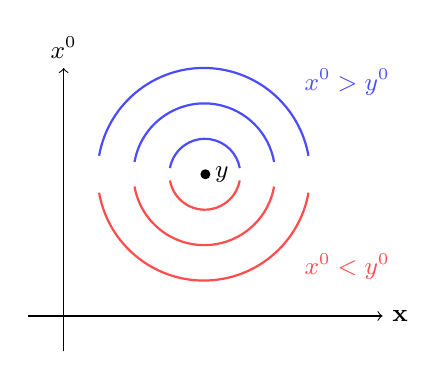
\begin{tikzpicture}[scale=0.9, every node/.style={font=\small}]
            \draw[->] (-0.5,0) -- (4.5,0) node[right] {$\mathbf{x}$};
            \draw[->] (0,-0.5) -- (0,3.5) node[above] {$x^0$};

            \coordinate (y) at (2,2);
            \fill (y) circle (2pt) node[right] {$y$};


            \foreach \r in {0.5,1.0,1.5} {
                    \pgfmathsetmacro{\yval}{\r*sin(10)};
                    \draw[blue!70, thick]
                    (y) ++(-\r, \yval) arc[start angle=170, end angle=10, radius=\r];
                }

            \foreach \r in {0.5,1.0,1.5} {
                    \pgfmathsetmacro{\yval}{\r*sin(10)};
                    \draw[red!70, thick]
                    (y) ++(-\r,-\yval) arc[start angle=190, end angle=350, radius=\r];
                }

            \node[blue!70] at (4,3.3) {$x^0 > y^0$};
            \node[red!70] at (4,0.7) {$x^0 < y^0$};
        \end{tikzpicture}
    \end{minipage}
\end{figure}

Other prescriptions to displace the poles lead to different Green functions satisfying (\eqref{eq:GF_def}), which we now rewrite as
\begin{equation}
    (-\Box_x + m^2) G(x - y) = \delta^4(x - y),
    \label{eq:41}
\end{equation}
with $y^\mu$ the spacetime point that supports the external source. The \textbf{retarded Green function} $G_R(x - y)$ is defined to propagate all frequencies excited by the source at the spacetime point $y^\mu$ forward in time, so that $G_R(x - y)$ vanishes for $x^0 < y^0$. It is fixed by displacing all the poles below the real $p^0$ axis. The \textbf{advanced Green function} $G_A(x - y)$ is defined to propagate all frequencies backward in time so that it vanishes for $x^0 > y^0$. It is obtained by displacing the poles above the real $p^0$ axis.

In the massless case ($m = 0$), and setting again $y^\mu = 0$ for simplicity, one computes the integrals and obtains
\begin{equation}
    G_R(x) = \frac{1}{4\pi r} \, \delta(t - r),
    \qquad
    G_A(x) = \frac{1}{4\pi r} \, \delta(t + r),
    \label{eq:42}
\end{equation}
where $t = x^0$ and $r = |\mathbf{x}|$, as known from electromagnetism. They can be written in a manifestly Lorentz-invariant form as
\begin{equation}
    G_R(x) = \frac{\theta(x^0)}{2\pi} \delta(x^2),
    \qquad
    G_A(x) = \frac{\theta(-x^0)}{2\pi} \delta(x^2).
    \label{eq:43}
\end{equation}

\paragraph{Real and virtual particle propagation.}
The propagator describes how field excitations travel through spacetime, encompassing both \textit{real} and \textit{virtual} particles.
Real particles correspond to on-shell modes satisfying the mass-shell condition \(p^2 = -m^2\), representing observable quanta that propagate over macroscopic distances.
\begin{figure}[H]
    \begin{minipage}{0.55\textwidth}
        Virtual particles, instead, are off-shell fluctuations (\(p^2 \neq -m^2\)) that exist only as intermediate states in interactions.
        Although they cannot be directly detected, their presence is essential: they mediate forces and account for quantum corrections in perturbation theory.
        Thus, the propagator unifies the causal motion of real particles and the short-lived virtual exchanges responsible for interactions.
    \end{minipage}
    \hfill
    \begin{minipage}{0.4\textwidth}
        \centering
        \begin{tikzpicture}[scale=1.2, thick,
                particle/.style={draw, postaction={decorate}, decoration={markings,mark=at position 0.55 with {\arrow{>}}}},
                photon/.style={decorate, decoration={snake, segment length=6pt, amplitude=2pt}},
                >=latex
            ]

            % incoming real particles (left)
            \draw[particle, green!60!black] (-2,1.2) -- (-0.5,0) node[midway, left] {$p_1$};
            \draw[particle, green!60!black] (-0.5,0) -- (-2,-1.2) node[midway, left] {$p_2$};

            % outgoing real particles (right)
            \draw[particle, yellow!80!black] (2,1.2) -- (0.5,0) node[midway, right] {$p_3$};
            \draw[particle, yellow!80!black] (0.5,0) -- (2,-1.2) node[midway, right] {$p_4$};

            % virtual photon propagator (horizontal wavy line)
            \draw[photon, gray] (-0.5,0) -- (0.5,0) node[midway, above] {$q$};

            % interaction vertices
            \filldraw[fill=white] (-0.5,0) circle (1.2pt);
            \filldraw[fill=white] (0.5,0) circle (1.2pt);

            % time axis
            \draw[->, thick] (-2.2,-1.8) -- (2.2,-1.8) node[right] {};
            \node at (0,-1.5) {$t$};
        \end{tikzpicture}
    \end{minipage}
\end{figure}



\paragraph{Exercise:} Derive the retarded and advanced Green functions in eqs.~(\eqref{eq:43}) by
performing the momentum integrations.

\paragraph{Exercise:} Derive the Yukawa potential by using the propagator and
eq.~(\eqref{eq:KG_solution_GF}), setting $\phi_0 = 0$ and $J(x) = -g \, \delta^3(\mathbf{x})$.

\subsubsection{Action}

The \textit{action principle} provides a compact and elegant way to express the dynamics of a physical system.
Rather than writing equations of motion directly, one defines a single functional quantity — the \textit{action} — whose stationary points correspond to the physical trajectories or field configurations that the system can take.
This principle plays a central role not only in classical field theory but also in quantum field theory, where it is essential for the formulation of the \textit{path integral quantization}.
A brief review of the action formalism and Noether’s theorem is given in Appendix \ref{app:Noether}.\TODO{Add appendix}

We can verify that the Klein--Gordon (KG) equation for a complex scalar field $\phi(x)$ follows from the action
\begin{equation}
    S[\phi, \phi^{\ast}] = \int \mathrm{d}^4 x \, \mathcal{L},
    \qquad
    \mathcal{L} = \left(- \partial_{\mu} \phi^{\ast} \partial^{\mu} \phi - m^2 \phi^{\ast} \phi \right),
    \label{eq:KG_action_lagrangian}
\end{equation}
where $\mathcal{L}$ is the \textit{Lagrangian density}, a local function of the fields and their derivatives.
It is the Lagrangian density that determines the equations of motion through the \textit{least action principle}, which states that the physical evolution of the field makes the action stationary under arbitrary infinitesimal variations of the fields:
\begin{equation}
    \delta S[\phi, \phi^{\ast}] \equiv S[\phi + \delta \phi, \phi^{\ast} + \delta \phi^{\ast}] - S[\phi, \phi^{\ast}] = 0.
    \label{eq:least_action_principle}
\end{equation}

By varying $\phi$ and $\phi^{\ast}$ independently and taking the variation inside the integral, one finds:
\[
    \begin{aligned}
        \delta S & = \int \mathrm{d}^4 x \left( - \partial_{\mu} \delta\phi^{\ast} \partial^{\mu} \phi- \partial_{\mu} \phi^{\ast} \partial^{\mu} \delta\phi -m^2 \delta \phi^{\ast} \phi -m^2 \phi^{\ast} \delta \phi \right) \\
                 & = \int \mathrm{d}^4 x \left[\delta \phi \left( - \partial^{\mu} \partial_{\mu} \phi^{\ast} -m^2 \phi^{\ast}\right)+\delta \phi^{\ast}\left( - \partial_{\mu} \partial^{\mu} \phi -m^2 \phi \right)\right].
    \end{aligned}
\]
Since the variations $\delta \phi$ and $\delta \phi^{\ast}$ are arbitrary, the integrand must vanish independently for each, leading to the Euler–Lagrange equations:
\[
    \begin{aligned}
        (\Box - m^2)\phi(x)        & = 0, \\
        (\Box - m^2)\phi(x)^{\ast} & = 0.
    \end{aligned}
\]
These are exactly the Klein--Gordon equations for a complex scalar field and its complex conjugate.

Alternatively, one can express the same result using \textit{functional derivatives}.
Writing the variation of the action as
\[
    \delta S[\phi, \phi^{\ast}] =
    \int \mathrm{d}^4 x \left(
    \frac{\delta S[\phi, \phi^{\ast}]}{\delta \phi(x)} \, \delta \phi(x)
    + \frac{\delta S[\phi, \phi^{\ast}]}{\delta \phi^{\ast}(x)} \, \delta \phi^{\ast}(x)
    \right) = 0,
\]
and imposing suitable boundary conditions (so that surface terms vanish), one obtains the field equations
\[
    \frac{\delta S[\phi, \phi^{\ast}]}{\delta \phi^{\ast}(x)} = (\Box - m^2)\phi(x) = 0,
    \qquad
    \frac{\delta S[\phi, \phi^{\ast}]}{\delta \phi(x)} = (\Box - m^2)\phi^{\ast}(x) = 0.
\]
This formulation is particularly useful in quantum field theory, where the action functional plays the role of the “generator” of the dynamics and symmetries of the theory.

For a \textit{real} scalar field $\phi = \phi^{\ast}$, the action is usually written with a conventional normalization factor:
\[
    S[\phi] = \int \mathrm{d}^4 x
    \left(
    -\frac{1}{2} \, \partial_{\mu} \phi \, \partial^{\mu} \phi
    - \frac{m^2}{2} \, \phi^2
    \right),
\]
from which we immediately obtain the equation of motion:
\[
    \frac{\delta S[\phi]}{\delta \phi(x)} = (\Box - m^2)\phi(x) = 0.
\]
This form highlights the direct analogy between a free scalar field and a collection of independent harmonic oscillators labeled by momentum.

Finally, note that a \textit{complex} scalar field can always be decomposed into two real fields of equal mass.
Setting
\[
    \phi = \frac{1}{\sqrt{2}}(\varphi_1 + i \varphi_2), \qquad
    \phi^{\ast} = \frac{1}{\sqrt{2}}(\varphi_1 - i \varphi_2),
\]
where $\varphi_1$ and $\varphi_2$ denote the real and imaginary parts of $\phi$, one finds that the Lagrangian density in \eqref{eq:KG_action_lagrangian} becomes
\begin{equation}
    \mathcal{L}
    = -\partial_{\mu}\phi^{\ast}\partial^{\mu}\phi - m^2\phi^{\ast}\phi
    = -\frac{1}{2}\partial_{\mu}\varphi_1\partial^{\mu}\varphi_1
    -\frac{1}{2}\partial_{\mu}\varphi_2\partial^{\mu}\varphi_2
    -\frac{m^2}{2}(\varphi_1^2 + \varphi_2^2).
    \label{eq:KG_real_lagrangian}
\end{equation}
Hence, a complex scalar field is dynamically equivalent to two independent real Klein--Gordon fields with identical masses.
This observation will be useful later when discussing internal symmetries and conserved currents.

\subsubsection{Symmetries}

The action formalism provides a powerful framework to connect \textit{symmetries} of a theory—i.e.\ transformations that leave the action invariant—with corresponding \textit{conservation laws}.
This fundamental relation is expressed by \textbf{Noether’s theorem}, reviewed in Appendix~\ref{app:Noether}.

The free complex Klein--Gordon field possesses two main types of rigid (or \textit{global}) symmetries:
1. **Space–time symmetries**, described by the \textit{Poincaré group}, and
2. **Internal symmetries**, associated with the invariance under phase rotations belonging to the group \(\mathrm{U}(1)\).

The term “rigid” (or equivalently “global”) indicates that these transformations do not depend on the spacetime point \(x\): the same transformation is applied everywhere, unlike in the case of \textit{gauge symmetries}, where the transformation parameters are local functions of \(x\).

\paragraph{The global \(\mathrm{U}(1)\) symmetry.}
The \(\mathrm{U}(1)\) symmetry corresponds to phase rotations of the field:
\begin{equation}
    \phi(x) \rightarrow \phi'(x) = e^{i\alpha} \phi(x),
    \qquad
    \phi^{\ast}(x) \rightarrow \phi'^{\ast}(x) = e^{-i\alpha} \phi^{\ast}(x),
    \label{eq:U1_symmetry}
\end{equation}
where \(\alpha\) is a real constant parameter.
It is straightforward to verify that under this transformation the action in \eqref{eq:KG_action_lagrangian} remains invariant:
\[
    S[\phi', \phi'^{\ast}] = S[\phi, \phi^{\ast}].
\]
In the real-field basis used in eq.~\eqref{eq:KG_real_lagrangian}, this symmetry corresponds to ordinary rotations in the plane spanned by \((\varphi_1, \varphi_2)\), i.e.\ to an \(\mathrm{SO}(2)\) symmetry.

For infinitesimal transformations (\(\alpha \ll 1\)), one can expand the exponentials and obtain:
\begin{equation}
    \delta_{\alpha}\phi(x) = \phi'(x) - \phi(x) = i\alpha \phi(x),
    \qquad
    \delta_{\alpha}\phi^{\ast}(x) = \phi'^{\ast}(x) - \phi^{\ast}(x) = -i\alpha \phi^{\ast}(x),
    \label{eq:U1_infinitesimal_transformations}
\end{equation}
which again leave the action invariant, \(\delta_{\alpha}S[\phi, \phi^{\ast}] = 0\).

\paragraph{From global to local transformations.}
If we now generalize the transformation parameter to depend on spacetime, \(\alpha \to \alpha(x)\), we obtain \textit{local} \(\mathrm{U}(1)\) transformations.
In this case, the action is no longer invariant, and the variation becomes
\begin{equation}
    \delta_{\alpha(x)} S[\phi, \phi^{\ast}] =
    \int \mathrm{d}^4 x \, \partial_{\mu}\alpha
    \underbrace{
        \left(
        i\phi^{\ast}\partial^{\mu}\phi
        - i(\partial^{\mu}\phi^{\ast})\phi
        \right)
    }_{J^{\mu}}.
    \label{eq:U1_variation}
\end{equation}
For a constant \(\alpha\), \(\partial_{\mu}\alpha = 0\) and the variation vanishes, confirming that the \(\mathrm{U}(1)\) symmetry is global.
The expression multiplying \(\partial_{\mu}\alpha\) identifies the conserved \textbf{Noether current}:
\begin{equation}
    J^{\mu} = i\phi^{\ast}\partial^{\mu}\phi - i(\partial^{\mu}\phi^{\ast})\phi
    \equiv i\phi^{\ast}\!\stackrel{\leftrightarrow}{\partial^{\mu}}\!\phi.
    \label{eq:U1_Noether_current}
\end{equation}
By applying the equations of motion, one verifies that this current satisfies the continuity equation
\[
    \partial_{\mu}J^{\mu} = 0.
\]
Indeed, since the equations of motion arise from \(\delta S = 0\) for arbitrary variations, the variation in \eqref{eq:U1_variation} must vanish for all possible choices of \(\alpha(x)\), implying \(\partial_{\mu}J^{\mu} = 0\).
This is precisely the mechanism behind Noether’s theorem.

The conserved \textbf{charge} associated with this current is
\begin{equation}
    Q \equiv \int d^3x \, J^0
    = -i \int d^3x \, \phi^{\ast}
    \!\stackrel{\leftrightarrow}{\partial_0}\!\phi,
    \label{eq:U1_Noether_charge}
\end{equation}
which is constant in time.
However, \(Q\) is not positive definite: this is why, in the context of the Klein--Gordon field, it cannot be interpreted as a probability.

Still, this structure motivates the definition of a \textit{conserved scalar product} between any two solutions \(\chi\) and \(\phi\) of the Klein--Gordon equation:
\[
    \langle \chi | \phi \rangle
    \equiv \int d^3x \, i \chi^{\ast}
    \!\stackrel{\leftrightarrow}{\partial_0}\!\phi.
\]
Using the equations of motion, one can verify that this inner product is time-independent.

\paragraph{Poincaré symmetries.}
The other fundamental symmetry of the Klein--Gordon theory is its invariance under the \textit{Poincaré group}, which combines Lorentz transformations and translations:
\begin{equation}
    x^{\mu} \rightarrow x'^{\mu} = \Lambda^{\mu}_{\ \nu} x^{\nu} + a^{\mu},
    \qquad
    \phi(x) \rightarrow \phi'(x') = \phi(x),
    \qquad
    \phi^{\ast}(x) \rightarrow \phi'^{\ast}(x') = \phi^{\ast}(x).
    \label{eq:Poincaré_symmetries}
\end{equation}
The field \(\phi\) thus transforms as a scalar under Poincaré transformations, and the action is easily verified to be invariant.

To extract the associated conserved quantities, it is convenient to study the \textit{infinitesimal} form of these transformations.
For an infinitesimal translation \(a^{\mu}\)
\[
    \begin{aligned}
        \delta_a \phi(x) & = \phi^{\prime} (x) - \phi(x) = \phi^{\prime} (x) - \phi^{\prime} (x^{\prime})                                                    \\
                         & = \delta_a \phi^{\prime} (x) = - \left(\phi^{\prime} (x+a) - \phi^{\prime} (x)\right)                                             \\
                         & = - \left(\phi^{\prime} (x) + a^{\mu}\delta_\mu \phi^{\prime}(x) - \phi^{\prime} (x)\right) = -a^{\mu}\delta_\mu \phi^{\prime}(x)
    \end{aligned}
\]\TODO{check calculationss}
where we have Taylor expanded, so that eq. \eqref{eq:Poincaré_symmetries} becomes
\begin{equation}
    \begin{aligned}
        \delta_a \phi(x)        & = -a^{\mu} \partial_{\mu} \phi(x),        \\
        \delta_a \phi^{\ast}(x) & = -a^{\mu} \partial_{\mu} \phi^{\ast}(x).
    \end{aligned}
    \label{eq:Poincaré_infinitesimal_transformations}
\end{equation}
If we let the parameter \(a^{\mu}\) depend arbitrarily on \(x\), Noether’s theorem yields the four corresponding conserved currents — in this case, the components of the \textbf{energy–momentum tensor}:
\[
    \delta_{a(x)} S[\phi, \phi^{\ast}]
    = \int \mathrm{d}^4 x \, (\partial_{\mu} a_{\nu})
    \underbrace{
        \left(
        \partial^{\mu}\phi^{\ast}\partial^{\nu}\phi
        + \partial^{\nu}\phi^{\ast}\partial^{\mu}\phi
        + \eta^{\mu\nu}\mathcal{L}
        \right)
    }_{T^{\mu\nu}}.
\]
Here, total derivatives have been neglected, and \(\mathcal{L}\) denotes the Lagrangian density from eq.~\eqref{eq:KG_action_lagrangian}.
This tensor is both symmetric and conserved,
\[
    \partial_{\mu}T^{\mu\nu} = 0,
\]
which, according to Noether’s theorem, implies the existence of conserved quantities associated with spacetime translations.

The corresponding conserved four-vector
\[
    P^{\mu} = \int d^3x \, T^{0\mu},
\]
represents the total \textbf{four-momentum} of the field.
Each component of \(P^{\mu}\) is linked to a specific symmetry:
\begin{itemize}
    \item The temporal component \(P^{0}\) is conserved in \textbf{time translations} and represents the total \textit{energy};
    \item The spatial components \(P^{i}\) (\(i = 1, 2, 3\)) is conserved in \textbf{spatial translations} and represent the components of the \textit{momentum vector}.
\end{itemize}

Explicitly, the \textit{local energy density} is given by\TODO{compute it}
\[
    T^{00} = \partial_0 \phi^{\ast}\partial_0 \phi
    + \vec{\nabla}\phi^{\ast} \cdot \vec{\nabla}\phi
    + m^2 \phi^{\ast}\phi,
\]
so that the total conserved energy reads
\[
    P^{0} \equiv E = \int d^3x \, T^{00}.
\]
This quantity is conserved in time and, for the Klein–Gordon field, it is manifestly \textit{positive definite}.
The three remaining components \(P^{i} = \int d^3x \, T^{0i}\) form the total momentum of the field, conserved under spatial translations.

These results illustrate how the action formalism and Noether’s theorem together provide a unified and systematic way to identify the conserved quantities associated with the fundamental symmetries of a field theory.